\documentclass[
	oneside,         	 %% Comente essa linha para imprimir frente e verso
	pagestart=firstchapter,
	capchap,
%	english,
%	french,
%	spanish,
	brazil	        %% Idioma principal 
]{abntbibufjf}

%\cftsetindents{figure}{0em}{4.6em}
%\renewcommand*{\cftfigureaftersnum}{\hfill \textendash \space \space} 
%%%\renewcommand*{\cftfigureaftersnum}{\space \textendash \space} 

%\pdfminorversion=7		% Retira Warning "pdflatex.exe PDF inclusion: found PDF version <1.7>, but at most version <1.5> allowed"

% formatação
\usepackage{lmodern}
\usepackage[T1]{fontenc}
\usepackage[utf8]{inputenc}
\usepackage{indentfirst}
\usepackage{setspace}
\usepackage{url}
\usepackage{pdfpages} % Para adicionar folha de pdf
\usepackage{lastpage}
%\usepackage[american]{babel}

%\usepackage{fontspec}
%\usepackage[brazil]{babel}

\usepackage{graphicx}
\usepackage{xcolor}
\usepackage{microtype}
\usepackage{epstopdf}

\usepackage{subcaption}

%--Pacotes Adicionados----------------------------

\usepackage{algorithm,algorithmic}

% pacote matemático
\usepackage{amsmath}                %pacote matemático da American Mathematical Society.
\usepackage{amsfonts}
\usepackage{amssymb}
\usepackage{amstext}
\usepackage{mathrsfs}             %pacote para fontes usadas em transformadas.
\usepackage{icomma}              %notação decimal com virgula.
\usepackage{bm}                     %bold math
\usepackage{steinmetz}           %insere notação de fasor para grandezas complexas
\usepackage{siunitx}               %Coloca no sistema de unidades internacional

\DeclareMathOperator{\sen}{sen}     %declara operador seno.
\DeclareMathOperator{\floor}{floor}  
\DeclareMathOperator{\ceil}{ceil} 

%tabelas
\usepackage{multirow}
\usepackage{booktabs}
\usepackage{makecell}             %espaçamento entre linhas
\usepackage{longtable}            %quebra de tabela entre páginas

%figura
\captionsetup[figure]{position=top}
\captionsetup[subfigure]{position=bottom}
\usepackage{pdflscape}			%Colocar a figura em paisagem
\usepackage{rotating}			%rotacionar a figura e a legenda
\usepackage{float}

\usepackage{pgfplots}
\usepackage{pgf-pie}
\usepackage{tikz}
\pgfplotsset{compat=1.18}

\usetikzlibrary{shapes.geometric, arrows, positioning}

\tikzstyle{box} = [rectangle, rounded corners, minimum width=2.5cm, minimum height=1cm, text centered, draw=black, fill=white]
\tikzstyle{short} = [rectangle, minimum width=2.5cm, minimum height=1cm, text centered, draw=black, fill=green!20]
\tikzstyle{medium} = [rectangle, minimum width=2.5cm, minimum height=1cm, text centered, draw=black, fill=yellow!20]
\tikzstyle{long} = [rectangle, minimum width=2.5cm, minimum height=1cm, text centered, draw=black, fill=red!20]
\tikzstyle{arrow} = [thick,->,>=stealth]


% listas
\usepackage{glossaries} 
\usepackage[printonlyused]{acronym} 		%Para criar lista de acrônimos
%\usepackage[nolist,nohyperlinks]{acronym}	%Para criar lista de acrônimos sem lista

\usepackage{etoolbox} % garante compatibilidade com redefine de ambientes

\renewcommand{\subfigureautorefname}{\figureautorefname}		%Utilizar o autoref
\renewcommand{\chapterautorefname}{Chapter}
\renewcommand{\sectionautorefname}{Section}
\renewcommand{\subsectionautorefname}{Subsection}

\DeclareSIUnit \watthour {Wh}
\DeclareSIUnit \voltampere {VA}
\DeclareSIUnit \reactivevoltampere {var}

% bibliografia
\usepackage[alf,abnt-emphasize=bf,abnt-etal-list=0, abnt-etal-text=it,abnt-etal-cite=3]{abntex2cite}	%% Citação mais arcaica, mas considerada como única aceitável para algumas institições
\usepackage{url6023}		%Consertar o <> devido a atualização da norma ABNT 6023

% citações e listas
\usepackage{verbatim}

%-----------------------------------------------------------------------------

%% Obs.: Alguns acentos foram omitidos.

\titulo{Um Método em Tempo Real para Estimação de Fasores Harmônicos Usando FFT e Interpolação B-Spline}
%\subtitulo{Digite o subtítulo do trabalho, somente os nomes próprios com letras iniciais maiúsculas} 

\autor{Ricardo Rodrigues Rapozo}
\autorR{Rapozo, Ricardo}

\local{Juiz de Fora} %%Digitar o nome da cidade
\dia{17} %%Digitar o dia da defesa
\mes{março} %%Escrever por extenso o mês da defesa
\ano{2026} %%Digitar o ano da defesa

\orientador[Orientador:]{Leandro Rodrigues Manso Silva} %%Se precisar, troque [Orientador:] por [Orientadora:]
\orientadorR{Silva, L. R, M.}
\orientadorTitulo{Prof. Dr.} %%Digitar, dentro de chaves {}, a titula\c{c}\~ao do(a) orientador(a). Por exemplo: Prof. Dr., Eng.

\coorientador[Coorientador:]{Marcelo Antônio Alves Lima} %% Comentar esta linha se nao tiver coorientador. Se precisar, troque por [Cooorientadora:]. 
\coorientadorR{Lima, A. A. L.} %% Comentar esta linha se n\~ao tiver coorientador.
\coorientadorTitulo{D. Sc..} %% Comentar esta linha se n\~ao tiver coorientador.

\instituicao{Universidade Federal de Juiz de Fora}
\faculdade{Faculdade de Engenharia} %%Digitar, dentro das chaves {}, o nome da faculdade ou do instituto.

\area{Sistemas Eletrônicos} %%Digitar, dentro das chaves {}, a área ou modalidade do curso.

\tipodocumento{2} %% Digitar 1, 2 ou 3 dentro das { }: 1-> TCC; 2-> Mestrado; 3-> Doutorado

\ifthenelse{\equal{\inseretipodocumento}{1}}
	{\programa{Coordenação do Curso de Engenharia Elétrica}}
	{\programa{Programa de Pós-Graduação em Engenharia Elétrica}}

\ifthenelse{\equal{\inseretipodocumento}{1}}
	{\objeto{Trabalho de Conclusão de Curso (Graduação)}}
	{\ifthenelse{\equal{\inseretipodocumento}{2}}
	{\objeto{Dissertação (Mestrado)}}
	{\objeto{Tese (Doutorado)}}
	}

\ifthenelse{\equal{\inseretipodocumento}{1}}
	{\natureza{Trabalho de Conclusão de Curso apresentado à \insereprograma ~da \insereinstituicao ~como requisito parcial à obtenção do grau de Bacharel em Engenharia Elétrica. Modalidade: \inserearea.}}
	{\ifthenelse{\equal{\inseretipodocumento}{2}}
	{\natureza{Dissertação apresentada ao \insereprograma ~da \insereinstituicao ~como requisito parcial à obtenção do título de Mestre em Engenharia Elétrica. Área: \inserearea.}}
	{\natureza{Tese apresentada ao \insereprograma ~da \insereinstituicao ~como requisito parcial à obtenção do título de Doutor em Engenharia Elétrica. Área: \inserearea.}}
	}

%% Abaixo, prencher com os dados da parte final da ficha catalografica

% Digitar as palavras-chaves no idioma Português  com letra inicial maiúscula.
\palavrachaveI{-} %% Digitar, dentro das { }, a primeira palavra-chave.
\palavrachaveII{-} %% Digitar, dentro das { }, a segunda palavra-chave.
\palavrachaveIII{-} %% Digitar, dentro das { }, a terceira palavra-chave.


% Digitar as palavras-chaves no idioma Inglês  com letra inicial maiúscula.
\keywordI{-} %% Digitar, dentro das { }, a primeira palavra-chave.
\keywordII{-} %% Digitar, dentro das { }, a segunda palavra-chave.
\keywordIII{-} %% Digitar, dentro das { }, a terceira palavra-chave.

\finalcatalog{1. \inserepalavrachaveI. 2. \inserepalavrachaveII. 3. \inserepalavrachaveIII. I. \insereorientadorR , orient. II. Título.}
\ifnotempty{\inserecoorientador}{
	\finalcatalog{1. \inserepalavrachaveI. 2. \inserepalavrachaveII. 3. \inserepalavrachaveIII. I. \insereorientadorR, orient. II. \inserecoorientadorR, coorient. III. Título.}}


\begin{document}

%% ELEMENTOS PRÉ-TEXTUAIS

%% Capa
\inserecapa

%% Folha de rosto
%\inserefolhaderosto

%% Ficha catalográfica. AO IMPRIMIR, DEIXAR NO VERSO DA FOLHA DE ROSTO.
\inserecatalog  


% Descomentar a próxima linha para inserir a folha de aprovação assinada eletronicamente
%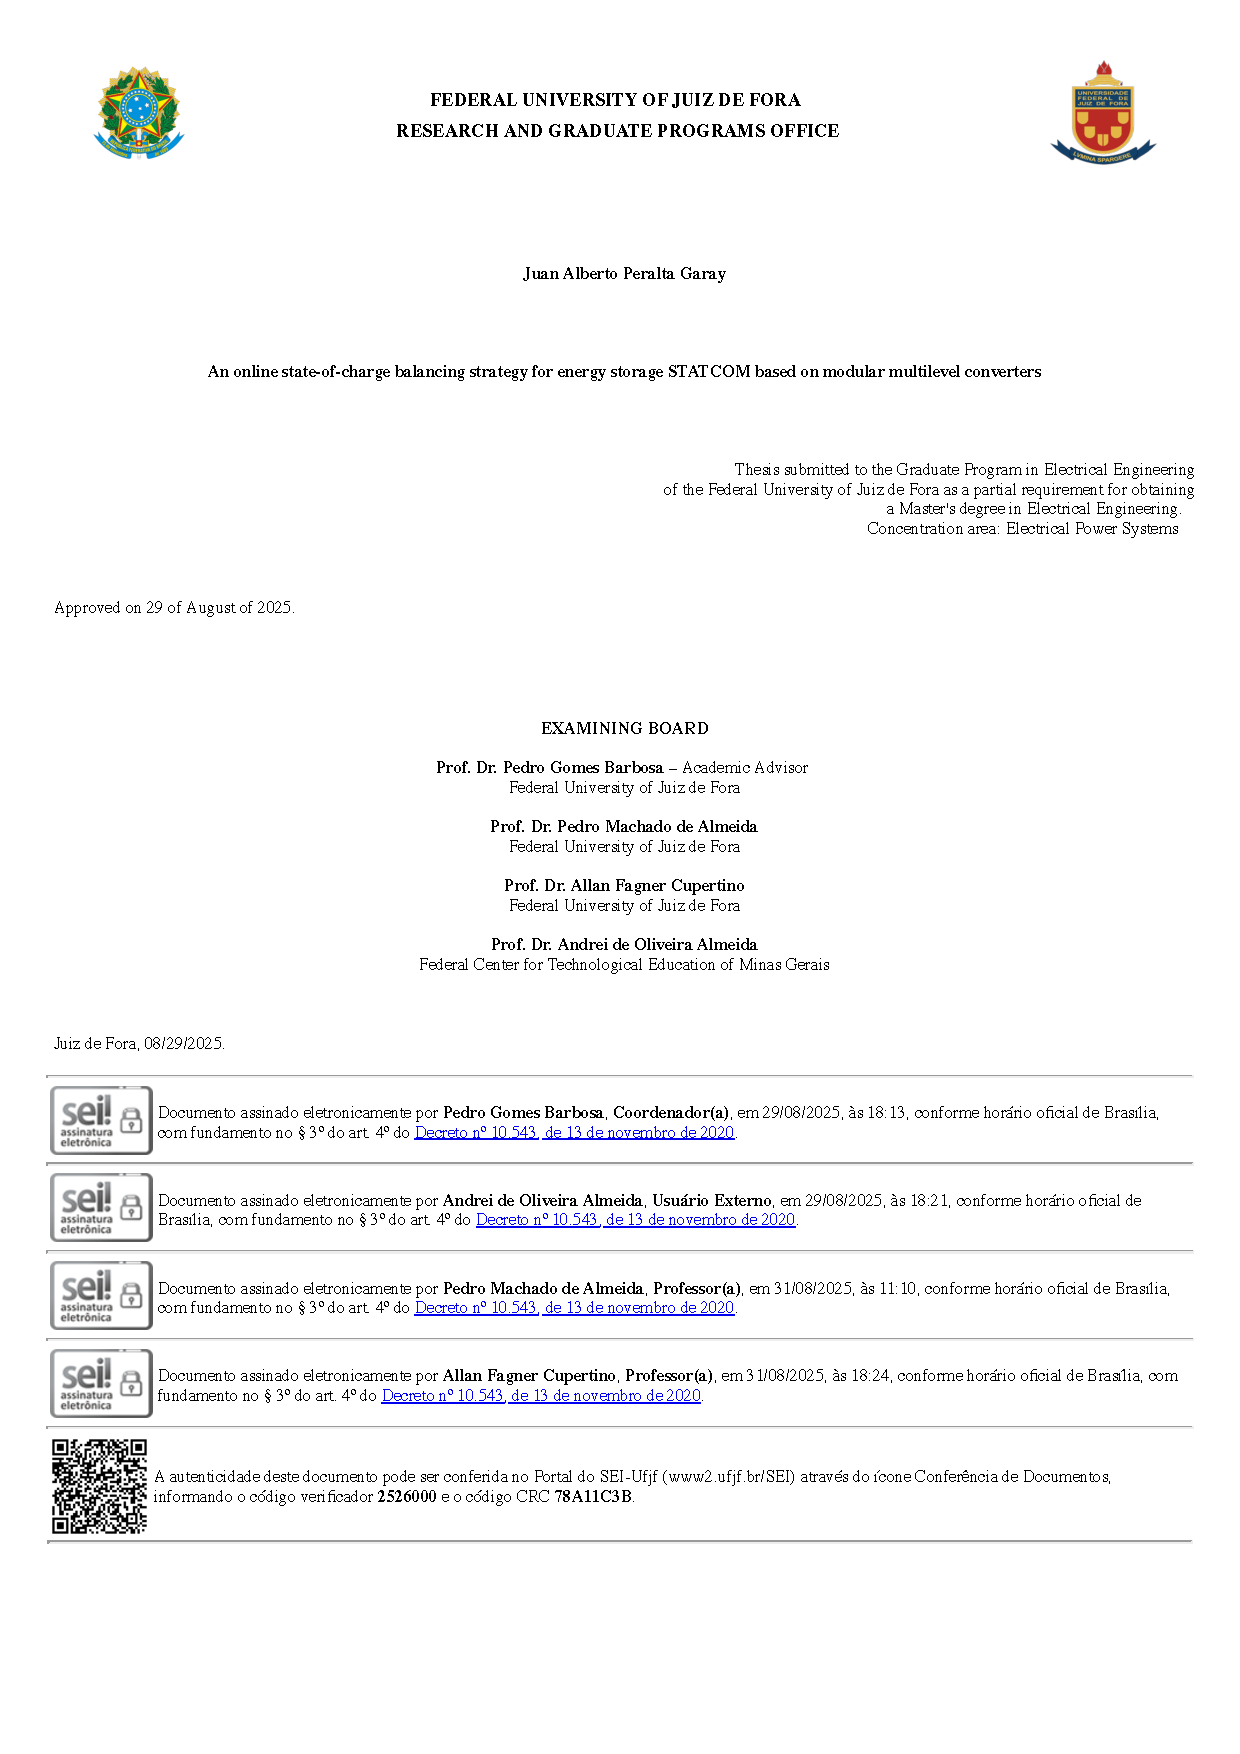
\includepdf{./Folha_Aprovacao.pdf} 
% Folha de aprovacao
\begin{folhadeaprovacao}
	\inicfolhaaprov
	
	Aprovada em \inseredia~de \inseremes~de \insereano. %%Preencher com a data 
	
	\vfill
	\begin{center} BANCA EXAMINADORA \end{center}
	\assinatura{\insereorientadorTitulo~\insereorientador \ - Orientador \\ Universidade Federal de Juiz de Fora - UFJF}  %%Orientadora
	{\ifnotempty{\inserecoorientador}{%
			{\assinatura{\inserecoorientadorTitulo~\inserecoorientador \ - Coorientador \\  Universidade Federal de Juiz de Fora - UFJF} \par }%
		}
	}
	\assinatura{Prof. Dr.- Henrique Luiz Moreira Monteiro \\ Universidade Federal de Labras - UFLA}
	\assinatura{Prof. Dr.- Carlos Augusto Duque \\ Universidade Federal de Juiz de Fora - UFJF}
\end{folhadeaprovacao}
\cleardoublepage 


%% Dedicatoria. OPCIONAL. Colocar ``%'' no início da próxima linha, caso não queira.
\begin{dedicatoria} 
  \textit{Dedico este trabalho -------.} %% substituir 
\end{dedicatoria}

%% Agradecimentos. OPCIONAL. CASO SEJA BOLSISTA, INSERIR OS DEVIDOS AGRADECIMENTOS.
\include{./pretextuais/agradecimentos}

%% Ep\'igrafe. OPCIONAL. Colocar ``%'' no início da próxima linha, caso não queira.
%\begin{epigrafe} 
	``\textit{-}''\\
	(-.
\end{epigrafe}


%% Resumo em Português. OBRIGATÓRIO.
\begin{resumo}

k

\textbf{Palavras-chave:} Estimação fasorial harmônica. Interpolação B-Spline. TVE-Erro Vetorial Total. FFT-Fast Fourier Transform.


\end{resumo}


%% Resumo em Inglês. OBRIGATÓRIO para teses e dissertações
\begin{otherlanguage*}{english}
\begin{resumo}[\textbf{ABSTRACT}]
.

\textbf{Keywords:} Harmonic phasor estimation. B-Spline interpolation. Total Vector Error (TVE). Fast Fourier Transform (FFT).

\end{resumo}
\end{otherlanguage*}



%% Lista de ilustra\c{c}\~oes. OPCIONAL.
\renewcommand{\listfigurename}{\textbf{LISTA DE FIGURAS}} 
\pdfbookmark[0]{\listfigurename}{lof}  
\listoffigures*
\cleardoublepage

%% Lista de tabelas. OPCIONAL. 
\renewcommand{\listtablename}{\textbf{LISTA DE TABELAS}} 
\pdfbookmark[0]{\listtablename}{lot}
\listoftables*    %Coloque ``%'' no in\'icio desta linha, caso n\~ao queira lista de tabelas.
\cleardoublepage

\chapter*{\textbf{LISTA DE ABREVIAÇÕES E ACRÔNIMOS}}
\begin{acronym}[ROCOF] %% Depois de rodar a primeira vez, digite entre os [ ] a sigla mais longa para justificar a lista de acrônimos à esquerda
\acro{AM}{Amplitude Modulation}
\acro{AR}{Autoregressive}
\acro{BS}{B-Spline}
\acro{DFT}{Discrete Fourier Transform}
\acro{FFT}{Fast Fourier Transform}
\acro{FIR}{Finite Impulse Response}
%\acro{Fs}{Sampling Frequency}
%\acro{f0}{Nominal Frequency}
%\acro{fm}{Modulation Frequency}
%\acro{H}{Number of Harmonics}
\acro{IEC}{International Electrotechnical Commission}
\acro{IEEE}{Institute of Electrical and Electronics Engineers}
%\acro{ka}{Phase Modulation Index}
%\acro{kx}{Amplitude Modulation Index}
%\acro{Nc}{Number of Cycles}
%\acro{Nppc}{Number of Points per Cycle}
\acro{PM}{Phase Modulation}
\acro{PMU}{Phasor Measurement Unit}
\acro{ROCOF}{Rate of Change of Frequency}
\acro{RMS}{Root Mean Square}
\acro{SNR}{Signal-to-Noise Ratio}
\acro{TFT}{Taylor-Fourier Transform}
\acro{TVE}{Total Vector Error}
\acro{WAMS}{Wide-Area Measurement Systems}
\acro{ZC}{Zero Crossing}
\acro{ZCD}{Zero Crossing Detector}

\end{acronym}



\renewenvironment{simbolos}
{
	\chapter*{\textbf{LISTA DE SÍMBOLOS}}
%	\addcontentsline{toc}{chapter}{List of Symbols}
	\begin{description}
	}{
	\end{description}
}

% Lista de s\'imbolos. OPCIONAL

\begin{simbolos} %%ALTERAR OS EXEMPLOS ABAIXO, CONFORME A NECESSIDADE
	
% \item[$????$] Description
\item[$f_0$] Frequência nominal.
\item[$f_m$] Frequência de modulação.
\item[$F_s$] Frequência de amostragem.
\item[$T_s$] Período de amostragem.
\item[$h$] Ordem harmônica.
\item[$H$] Número total de harmônicos.
\item[$A_h$] Amplitude do harmônico de ordem $h$.
\item[$\phi_{0h}$] Fase inicial do harmônico de ordem $h$.
\item[$k_x$] Índice de modulação em amplitude.
\item[$k_a$] Índice de modulação em fase.
\item[$ X_{h[n]} $] Fasor harmônico de referência.
\item[$\lambda$] Fator de reamostragem ($\lambda = f_{\text{ref}}/f_{\text{inst}}$).
\item[\ensuremath{\nu[n]}] Ruído aditivo.
\item[$A_{\mathrm{RMS}}$] Valor eficaz da amplitude.
\item[$n$] Índice discreto.
\item[$t$] Variável temporal contínua.

\end{simbolos}






 
%% Sum\'ario
\renewcommand{\contentsname}{\textbf{CONTEÚDO}}
\pdfbookmark[0]{\contentsname}{toc}
\tableofcontents*
\cleardoublepage

%% ELEMENTOS TEXTUAIS
\textual

\acresetall

\chapter{Introdução}\label{cap:intro}

A operação de redes elétricas modernas envolve sinais cada vez menos próximos do modelo senoidal ideal. Conversores eletrônicos, cargas não lineares, geração distribuída, sistemas de armazenamento e fontes renováveis conectadas por eletrônica de potência alteram a forma de onda de tensões e correntes, introduzindo componentes harmônicas, variações de amplitude, desvios de frequência e ruído. Nesse cenário, a análise apenas da componente fundamental pode ser insuficiente para caracterizar o estado do sistema e para apoiar aplicações de qualidade de energia, diagnóstico de distorções e monitoramento em tempo real.

A estimação fasorial sincronizada tornou-se uma ferramenta importante para a observação de Sistemas Elétricos de Potência, pois associa grandezas elétricas medidas em diferentes pontos a uma base temporal comum. As PMUs (\textit{Phasor Measurement Units}) são capazes de estimar fasores, frequência e ROCOF da componente fundamental, permitindo comparar medições obtidas em locais distintos da rede \cite{phadke2008,ieee2011}. Entretanto, a extensão desse conceito para componentes harmônicas ainda é menos consolidada. Enquanto os sincrofasores da fundamental possuem requisitos normativos bem definidos, a estimação sincronizada de fasores harmônicos ainda carece de padronização completa, especialmente no que diz respeito a ensaios, limites de erro e condições dinâmicas \cite{iec60255}.

Essa lacuna é relevante porque os harmônicos não apenas acrescentam componentes espectrais ao sinal; eles também tornam mais sensível o problema de sincronismo temporal. Quando a frequência fundamental se afasta da nominal, filtros e janelas projetados para uma grade fixa passam a observar o sinal em instantes ligeiramente desalinhados. Esse desalinhamento produz erro de magnitude e, principalmente, erro de fase. Em componentes harmônicas, o efeito angular se torna mais crítico, pois a fase associada à ordem $h$ evolui $h$ vezes mais rapidamente que a fase da fundamental. Assim, pequenas imprecisões na frequência estimada, nos atrasos de processamento ou nos instantes de amostragem podem gerar erros expressivos nas ordens mais elevadas.

Outro aspecto importante é o custo computacional. Bancos de filtros são atrativos para estimação harmônica por permitirem extrair simultaneamente várias componentes, mas a implementação direta de um filtro para cada harmônico pode exigir grande número de operações. Esse custo se torna um obstáculo quando se deseja monitorar muitas ordens harmônicas ou quando a implementação deve operar em plataformas embarcadas. A decomposição polifásica oferece uma forma de reorganizar o banco de filtros e reduzir a carga computacional, preservando a interpretação de filtragem multicanal \cite{mk06}. Em paralelo, filtros Flat-Top são interessantes por apresentarem resposta de magnitude plana ao redor da frequência central, característica útil para reduzir a sensibilidade da estimação a pequenos desvios de frequência \cite{duda2019}.

Além da extração harmônica propriamente dita, é necessário lidar com a variação da frequência fundamental antes que o sinal chegue ao banco de filtros. Uma alternativa é reprojetar ou selecionar filtros de acordo com a frequência estimada, mas essa estratégia pode aumentar a complexidade da implementação. Outra possibilidade é reamostrar dinamicamente o sinal, gerando amostras em instantes compatíveis com o período elétrico estimado. Nesse caso, o banco posterior continua operando em uma base nominal, enquanto a adaptação à frequência real ocorre na etapa de interpolação. A interpolação B-Spline, implementada por estrutura de Farrow, é uma alternativa adequada para esse tipo de reamostragem por permitir a geração de amostras em posições fracionárias com coeficientes fixos \cite{aleixo2022}.

Este trabalho investiga uma metodologia de estimação de fasores harmônicos que combina três elementos principais: estimação da frequência fundamental por cruzamento por zero, reamostragem dinâmica por interpolação B-Spline e extração harmônica por banco de filtros Flat-Top com decomposição polifásica. A proposta é formulada com foco em uma implementação futura em FPGA com processadores \textit{soft-core}, mas a validação final em hardware e os resultados completos de desempenho não são tratados como concluídos nesta etapa. A dissertação, portanto, concentra-se na fundamentação, na organização metodológica e na preparação da cadeia de processamento que será avaliada experimentalmente em etapa posterior.

\section{Motivação}

A motivação deste trabalho surge da necessidade de estimadores harmônicos que sejam, ao mesmo tempo, precisos e viáveis para implementação embarcada. Em um cenário prático, o sinal medido pode apresentar ruído, distorção, desvio de frequência, rampas e modulações. Um estimador útil não deve depender apenas de condições estacionárias ideais; ele precisa preservar coerência de fase e magnitude mesmo quando a frequência fundamental se desloca da nominal.

O uso de reamostragem dinâmica é motivado por esse ponto. Se o sinal está, por exemplo, em frequência diferente da nominal, uma janela fixa deixa de representar exatamente o mesmo intervalo elétrico. A etapa de interpolação busca corrigir essa incompatibilidade temporal antes da extração dos fasores, reduzindo o erro causado por analisar o sinal em uma grade inadequada. Com isso, o banco de filtros pode ser mantido em uma estrutura nominal, simplificando o processamento posterior.

A segunda motivação está ligada ao custo computacional da estimação multiharmônica. Monitorar várias ordens harmônicas por filtros independentes pode ser custoso, especialmente quando se considera uma implementação em tempo real. A decomposição polifásica é adotada como estratégia para tornar o banco de filtros mais eficiente, enquanto o filtro Flat-Top é empregado pela sua característica de baixa sensibilidade de magnitude nas proximidades da frequência de interesse. O interesse central do trabalho está na integração dessas técnicas em uma mesma cadeia de estimação.

\section{Objetivos}

O objetivo geral deste trabalho é desenvolver uma metodologia para estimação de fasores harmônicos em sinais com frequência fundamental variável, combinando estimação de frequência por cruzamento por zero, reamostragem por interpolação B-Spline e banco de filtros Flat-Top com decomposição polifásica, com direcionamento para implementação futura em FPGA.

\subsection{Objetivos específicos}

Os objetivos específicos deste trabalho são:

\begin{itemize}
    \item estudar a representação de fasores, sincrofasores e fasores harmônicos no contexto de sinais elétricos com frequência variável;
    \item discutir métricas e ensaios usados em PMUs, utilizando a IEC/IEEE 60255-118-1 como referência metodológica para a construção de cenários de teste;
    \item formular a etapa de estimação de frequência por cruzamento por zero, incluindo filtragem preliminar, interpolação do instante de cruzamento e suavização da estimativa;
    \item explicar o papel do alinhamento temporal entre sinal, frequência estimada, filtros e interpolador;
    \item aplicar interpolação B-Spline em estrutura de Farrow para realizar a reamostragem dinâmica do sinal;
    \item organizar a extração dos fasores harmônicos por meio de um banco de filtros Flat-Top;
    \item empregar decomposição polifásica para reduzir o custo computacional associado ao banco de filtros;
    \item definir as métricas que serão usadas na validação posterior, incluindo TVE, erro de magnitude, erro de fase, erro de frequência e erro de ROCOF;
    \item estruturar a metodologia de forma compatível com uma implementação futura em FPGA com processadores \textit{soft-core}.
\end{itemize}

\section{Contribuições esperadas}

As principais contribuições esperadas deste trabalho são:

\begin{itemize}
    \item a organização de uma cadeia de estimação harmônica que integra rastreamento de frequência, reamostragem B-Spline e banco Flat-Top polifásico;
    \item a explicação do papel da reamostragem dinâmica na redução do desalinhamento temporal provocado por frequência fora da nominal;
    \item a formulação das etapas de atraso e alinhamento necessárias para manter coerência entre a frequência estimada e o trecho de sinal reamostrado;
    \item a adaptação de sinais de teste inspirados na IEC/IEEE 60255-118-1 para análise de componentes harmônicas;
    \item a preparação de uma descrição metodológica adequada para implementação e validação em FPGA em etapa posterior.
\end{itemize}

Como a implementação em FPGA ainda está em desenvolvimento, as contribuições desta etapa não são apresentadas como resultados finais de desempenho. O foco está na construção consistente do método, na conexão entre os blocos de processamento e na definição das condições que permitirão avaliar o estimador de forma organizada quando a implementação estiver consolidada.

\section{Divisão do trabalho}

O restante desta dissertação está organizado da seguinte forma.

O Capítulo~\ref{cap:cap2} apresenta a revisão bibliográfica e a fundamentação teórica. São discutidos fasores, sincrofasores, estimação fasorial, fasores harmônicos, normas e métricas de avaliação, interpolação, B-Splines, estrutura de Farrow, filtros Flat-Top e decomposição polifásica.

O Capítulo~\ref{cap:tres} descreve a metodologia proposta. Nesse capítulo, os conceitos apresentados separadamente na fundamentação são integrados em uma cadeia composta por estimação de frequência, suavização, alinhamento temporal, reamostragem dinâmica, banco de filtros polifásico, correção de fase e métricas de avaliação.

O Capítulo~\ref{cap:quatro} é reservado para resultados e discussões. Essa etapa deverá reunir, quando consolidados, os ensaios em condições estacionárias e dinâmicas, bem como a análise dos erros obtidos na estimação dos fasores harmônicos.

Por fim, a conclusão sintetiza os principais pontos desenvolvidos, discute limitações da etapa atual e indica os próximos passos relacionados à implementação em FPGA e à validação experimental do método.

\chapter{Revisão Bibliográfica e Fundamentação Teórica}\label{cap:cap2}

Este capítulo apresenta os conceitos necessários para o desenvolvimento da metodologia proposta. Inicialmente são discutidas as representações fasorial e sincrofasorial, pois elas definem a forma como sinais elétricos senoidais são descritos por magnitude e fase. Em seguida, são abordados os fasores harmônicos, as métricas de avaliação estabelecidas para PMUs e as limitações decorrentes de frequência variável. Por fim, são apresentados os fundamentos de interpolação B-Spline, estrutura de Farrow, filtros Flat-Top e decomposição polifásica, que formam a base técnica do método descrito no Capítulo~\ref{cap:tres}.

\section{Fasores}

Um fasor é uma representação complexa de uma grandeza senoidal em regime permanente. Essa representação é amplamente utilizada em sistemas elétricos porque permite substituir a descrição temporal completa de uma senoide por duas informações principais: magnitude e ângulo de fase. Com isso, a análise de circuitos e sistemas em corrente alternada torna-se mais simples, uma vez que a dependência temporal associada à frequência fundamental é separada da representação complexa da grandeza \cite{phadke2008}.

Considere o sinal senoidal

\begin{equation}
x(t) = X_m\cos(\omega t + \varphi),
\label{eq:cap2_sinal_senoidal}
\end{equation}

\noindent em que $X_m$ é a amplitude de pico, $\omega$ é a frequência angular e $\varphi$ é o ângulo de fase em relação a uma referência temporal. O valor eficaz associado à senoide é $X_m/\sqrt{2}$. Assim, o fasor correspondente pode ser escrito como

\begin{equation}
\bar{X} = \frac{X_m}{\sqrt{2}}e^{j\varphi}.
\label{eq:cap2_fasor}
\end{equation}

Na forma polar, a mesma grandeza é representada por

\begin{equation}
\bar{X} = X_{rms}\angle\varphi,
\label{eq:cap2_fasor_polar}
\end{equation}

\noindent em que $X_{rms}$ é o valor eficaz da grandeza. A informação temporal $\omega t$ não aparece explicitamente no fasor, pois a representação assume uma frequência de referência conhecida. Assim, o fasor convencional não descreve diretamente a evolução temporal do sinal; ele representa o módulo e o atraso angular da senoide em relação à referência adotada. Essa característica é adequada para regime permanente, mas torna-se mais delicada quando a frequência varia ao longo do tempo.

A Figura~\ref{fig:fasor} ilustra a relação entre uma senoide e sua representação no plano complexo. O ângulo do fasor indica a defasagem em relação à referência adotada, enquanto seu módulo está associado ao valor eficaz do sinal.

\begin{figure}[H]
    \centering
    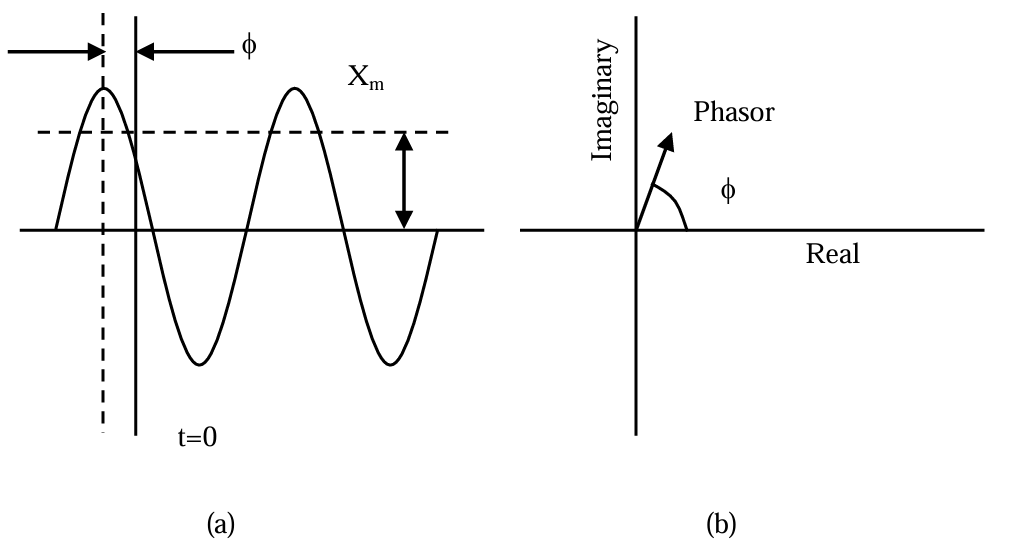
\includegraphics[scale=0.6]{textuais/capitulo2/imagens_capitulo_2/fasor_senoide.png}
    \caption{Representação de uma senoide e de seu fasor associado no plano complexo, adaptada de \cite{phadke2008}.}
    \label{fig:fasor}
\end{figure}

\section{Sincrofasores e PMUs}

Um sincrofasor é um fasor associado a uma referência temporal comum. Essa referência permite que medições realizadas em pontos geograficamente distintos de um sistema elétrico sejam comparadas de forma coerente. Em sistemas de medição fasorial sincronizada, essa base temporal é normalmente fornecida por sistemas de sincronização de alta precisão, como GPS, e utilizada por unidades de medição fasorial, conhecidas como PMUs (\textit{Phasor Measurement Units}) \cite{phadke2008,ieee2011}.

A principal diferença entre um fasor convencional e um sincrofasor está na associação explícita com uma estampa de tempo. Como o ângulo de fase depende do instante escolhido como referência, duas medições só podem ser comparadas de forma direta se estiverem sincronizadas. A vantagem prática dessa representação é permitir que fasores medidos em barras distintas sejam tratados como observações de um mesmo estado elétrico, preservando a coerência angular entre pontos afastados do sistema. Esse aspecto é fundamental em aplicações de monitoramento de grandes áreas, estimação de estado, proteção, controle e análise dinâmica de sistemas elétricos \cite{phadke2008,martins2012smfs}.

A Figura~\ref{fig:fasores_diversos} apresenta uma representação simplificada de medições fasoriais sincronizadas em diferentes pontos de um sistema elétrico. Na imagem, cada unidade de medição fornece um fasor local de tensão ou corrente, mas todos os ângulos são referidos à mesma base temporal. A existência dessa referência comum permite comparar os ângulos obtidos em barras distintas e relacioná-los ao estado operativo da rede.

\begin{figure}[H]
    \centering
    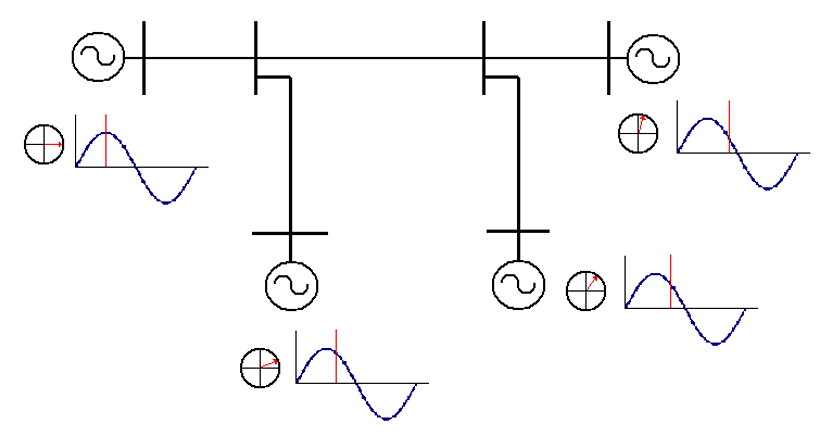
\includegraphics[scale=0.6]{textuais/capitulo2/imagens_capitulo_2/diferentes_fasores.png}
    \caption{Representação de medições fasoriais sincronizadas em diferentes pontos do sistema elétrico, adaptada de \cite{martins2012smfs}.}
    \label{fig:fasores_diversos}
\end{figure}

De forma geral, uma PMU realiza a aquisição dos sinais de tensão e corrente, aplica etapas de condicionamento e processamento digital, estima fasores, frequência e taxa de variação da frequência, e envia essas informações a um concentrador de dados fasoriais, ou PDC (\textit{Phasor Data Concentrator}). Esse arranjo é ilustrado na Figura~\ref{fig:PMU_max}.

\begin{figure}[H]
    \centering
    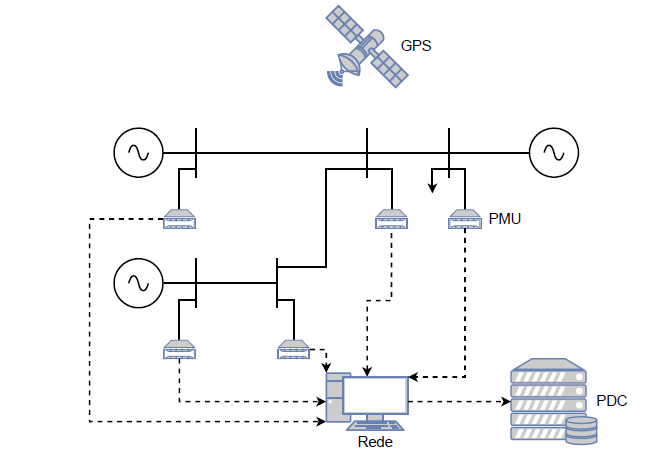
\includegraphics[scale=0.6]{textuais/capitulo2/imagens_capitulo_2/pmu_max.png}
    \caption{Estrutura geral de um sistema de medição fasorial sincronizada, adaptada de \cite{luiz2024qualificacao}.}
    \label{fig:PMU_max}
\end{figure}

\section{Estimação fasorial}

Na prática, os fasores não são obtidos a partir de expressões analíticas contínuas, mas por meio de sinais discretos adquiridos por conversores analógico-digitais. O problema da estimação fasorial consiste, portanto, em estimar magnitude, fase, frequência e, quando necessário, ROCOF a partir de um conjunto finito de amostras.

Entre as técnicas clássicas de estimação fasorial estão métodos baseados na DFT (\textit{Discrete Fourier Transform}), FFT (\textit{Fast Fourier Transform}), filtros digitais, PLLs, filtros de Kalman, métodos baseados em mínimos quadrados, Transformada de Taylor-Fourier e algoritmos interpolados no domínio da frequência. Cada família de métodos apresenta compromissos próprios entre precisão, tempo de resposta, robustez a ruído, rejeição de interferências e custo computacional.

Em condições estacionárias e com frequência nominal, métodos baseados na DFT tendem a apresentar boa precisão e implementação simples. Entretanto, quando a frequência do sinal se desvia da frequência nominal, a janela de observação deixa de conter um número inteiro de ciclos. Esse desalinhamento provoca espalhamento espectral e afeta a estimação da magnitude e da fase \cite{phadke2008,harris78}. O problema se torna ainda mais relevante em aplicações harmônicas, pois o erro de tempo ou de fase aparece no argumento das componentes em múltiplos da frequência fundamental. Assim, uma mesma incerteza angular associada à base temporal da fundamental tende a produzir efeito mais severo nas componentes de ordem elevada. Esse comportamento está no contexto dos desafios tratados em métodos de estimação de fasores harmônicos sob frequência variável \cite{duda2019,aleixo2022}.

Essa dificuldade pode ser vista diretamente a partir do referencial síncrono usado na definição fasorial. Considere uma senoide de valor eficaz $X_{\mathrm{rms}}$, frequência angular real $\omega$ e fase inicial $\varphi$,

\begin{equation}
x(t)=\sqrt{2}X_{\mathrm{rms}}\cos(\omega t+\varphi).
\label{eq:cap2_senoide_freq_real}
\end{equation}

\noindent Se a referência síncrona gira na frequência nominal $\omega_0$, a componente complexa associada ao sinal, observada nesse referencial, pode ser escrita como

\begin{equation}
\bar{X}(t)=X_{\mathrm{rms}}e^{j[(\omega-\omega_0)t+\varphi]}.
\label{eq:cap2_fasor_referencial_sincrono}
\end{equation}

\noindent Quando $\omega=\omega_0$, o termo dependente do tempo desaparece e o fasor permanece parado no referencial síncrono, com ângulo constante $\varphi$. Porém, quando $\omega\neq\omega_0$, surge uma rotação residual dada por

\begin{equation}
\varphi(t)=(\omega-\omega_0)t+\varphi.
\label{eq:cap2_fase_residual_freq}
\end{equation}

\noindent Portanto, a frequência fora da nominal não produz apenas um erro estático: ela faz o ângulo estimado variar ao longo da janela de observação. Em um estimador projetado para a base nominal, essa rotação residual aparece como deriva de fase e contribui para erros de magnitude e fase. Para componentes harmônicas, o mesmo raciocínio se torna mais crítico, pois a diferença angular é escalada pela ordem harmônica.

Esse contexto motiva o uso de técnicas que adaptem a análise à frequência real do sinal. Uma alternativa é reprojetar filtros sempre que a frequência muda. Outra possibilidade é reamostrar dinamicamente o sinal, de modo que o estimador posterior continue operando em uma base nominal. A metodologia deste trabalho segue a segunda abordagem, combinando estimação de frequência por cruzamento por zero e interpolação B-Spline para alimentar um banco de filtros harmônicos.

Nesse procedimento, as amostras originais continuam sendo adquiridas no relógio fixo do conversor analógico-digital. A partir dos cruzamentos por zero, estima-se o período elétrico real do sinal e calcula-se em quais instantes ele deveria ser observado para que cada ciclo fique compatível com a base nominal usada pelo estimador. Como esses instantes corrigidos geralmente caem entre duas amostras físicas, a interpolação B-Spline reconstrói o valor do sinal em posições fracionárias. Dessa forma, o método não altera o fenômeno medido; ele ajusta a base temporal entregue ao estimador. Uma componente que pareceria adiantada ou atrasada por causa do desvio de frequência passa a ser apresentada ao banco de filtros em instantes mais coerentes com a fase elétrica estimada. Os atrasos introduzidos pelos filtros e pelas etapas de média e interpolação são então compensados para que o fasor final permaneça referido ao instante correto.

\section{Fasores harmônicos}\label{sec:fasores_harmonicos}

Sinais elétricos reais podem conter componentes harmônicas decorrentes de cargas não lineares, conversores eletrônicos, saturação de equipamentos e outras fontes de distorção. Um sinal periódico não puramente senoidal pode ser representado como uma soma de componentes em múltiplos inteiros da frequência fundamental. Considerando uma frequência fundamental $f_1$, e seguindo a forma geral de sinais de ensaio adotada na IEC/IEEE 60255-118-1 \cite{iec60255}, uma representação simplificada é

\begin{equation}
x(t) = A_1\cos(2\pi f_1t + \varphi_1)
+ \sum_{h=2}^{H} A_h\cos(2\pi hf_1t + \varphi_h),
\label{eq:cap2_sinal_harmonicos}
\end{equation}

\noindent em que $h$ representa a ordem harmônica. O fasor associado à componente de ordem $h$ pode ser escrito como

\begin{equation}
\bar{X}_h = \frac{A_h}{\sqrt{2}}e^{j\varphi_h}.
\label{eq:cap2_fasor_harmonico}
\end{equation}

Quando a frequência fundamental varia, a fase da componente harmônica também passa a depender da trajetória temporal da frequência. Nesse caso, a fase instantânea da componente de ordem $h$ pode ser relacionada à fase da fundamental por

\begin{equation}
\theta_h(t) = h\theta_1(t) + \varphi_h.
\label{eq:cap2_fase_harmonico}
\end{equation}

Essa relação mostra por que a estimação de fasores harmônicos é sensível ao erro de frequência e ao desalinhamento temporal. Um pequeno erro na fase da componente fundamental tende a produzir erro proporcionalmente maior nas componentes de ordem elevada. Assim, técnicas de estimação harmônica precisam lidar simultaneamente com seletividade em frequência, precisão de fase e custo computacional.

A estimação sincronizada de fasores harmônicos ainda é um tema em desenvolvimento. Há aplicações potenciais em monitoramento de qualidade de energia, estimação de estado harmônico, localização de fontes de distorção, avaliação de filtros ativos e diagnóstico de fenômenos em redes com elevada penetração de eletrônica de potência. No entanto, diferentemente dos sincrofasores da componente fundamental, ainda não existe uma padronização ampla e consolidada para todos os requisitos de desempenho aplicáveis a HPMUs.

\section{Normas e métricas de avaliação}

As normas IEEE C37.118.1 e IEC/IEEE 60255-118-1 definem requisitos de desempenho para PMUs na estimação de sincrofasores, frequência e ROCOF da componente fundamental \cite{ieee2011,ieee2014,iec60255}. Essas normas estabelecem ensaios para condições estacionárias e dinâmicas, incluindo frequência fora da nominal, rampa de frequência, modulação de amplitude e modulação de fase.

Embora esses documentos não estabeleçam uma norma completa para fasores harmônicos, seus ensaios são úteis como referência metodológica. Neste trabalho, os cenários normativos são utilizados como base para construir sinais de teste contendo componentes harmônicas. Dessa forma, avalia-se o comportamento do método em condições compatíveis com aquelas usadas em PMUs, mas sem afirmar que a norma define todos os limites aplicáveis aos fasores harmônicos.

A métrica mais utilizada para avaliação fasorial é o TVE (\textit{Total Vector Error}), que compara o fasor estimado com o fasor de referência no plano complexo. Na IEC/IEEE 60255-118-1, essa métrica é definida por \cite{iec60255}

\begin{equation}
TVE =
100
\sqrt{
\frac{
\left(\hat{X}_r-X_r\right)^2+
\left(\hat{X}_i-X_i\right)^2
}{
X_r^2+X_i^2
}
},
\label{eq:cap2_tve}
\end{equation}

\noindent em que $\hat{X}_r$ e $\hat{X}_i$ são as partes real e imaginária do fasor estimado, e $X_r$ e $X_i$ são as partes real e imaginária do fasor de referência.

Além do TVE, a norma IEC/IEEE 60255-118-1 define o erro de frequência, dado por \cite{iec60255}

\begin{equation}
FE = \hat{f} - f,
\label{eq:cap2_fe}
\end{equation}

\noindent e o erro de ROCOF,

\begin{equation}
RFE = \widehat{ROCOF} - ROCOF.
\label{eq:cap2_rfe}
\end{equation}

Para interpretar o desempenho de estimadores harmônicos, também é útil separar o erro de magnitude e o erro de fase. O erro de magnitude indica a diferença entre os módulos dos fasores, enquanto o erro de fase indica o desalinhamento angular. Essa separação é importante porque dois estimadores podem apresentar TVE semelhante, mas por razões distintas: um pode ser limitado por erro de ganho, enquanto outro pode ser limitado por erro de fase.

\section{Interpolação e reamostragem dinâmica}

Uma estratégia para lidar com variação de frequência é reamostrar o sinal de entrada antes da estimação fasorial. A ideia é transformar uma sequência adquirida em taxa fixa em uma nova sequência cujos instantes estejam coerentes com a frequência estimada do sinal. Assim, em vez de alterar continuamente os filtros de extração harmônica, adapta-se a base temporal do sinal que alimenta esses filtros.

O ponto central é que a reamostragem não apenas aumenta ou reduz um buffer de amostras. Ela constrói uma nova grade de instantes para que o sinal seja observado de acordo com o período elétrico estimado. A fase inicial do sinal não é eliminada, pois ela faz parte do fasor que se deseja medir. O que se corrige é o descompasso acumulativo entre a grade temporal nominal e a frequência real do sinal. Em outras palavras, uma onda de \SI{61}{Hz} não deve ser forçada a ter fase de uma onda de \SI{60}{Hz}; ela deve ser entregue ao estimador em instantes tais que um ciclo real de \SI{61}{Hz} corresponda ao número nominal de amostras por ciclo usado pelo banco de filtros.

Considere que a taxa de aquisição seja $F_s=f_0N_{ppc}$, em que $N_{ppc}$ é o número nominal de pontos por ciclo. A aquisição original continua ocorrendo em taxa fixa, nos instantes $t_n=n/F_s$. A reamostragem não altera essa taxa de aquisição; ela apenas define uma nova grade de instantes $t_i[k]$ nos quais o sinal já adquirido será avaliado por interpolação.

Se o estimador posterior opera assumindo $N_{ppc}$ amostras por ciclo, então duas amostras consecutivas da sequência reamostrada devem estar separadas por $1/N_{ppc}$ do ciclo elétrico estimado. Como o período estimado é $1/\hat{f}[k]$, o avanço temporal desejado entre duas amostras interpoladas é

\begin{equation}
t_i[k+1] = t_i[k] + \frac{1}{N_{ppc}\hat{f}[k]}.
\label{eq:cap2_tempo_interpolado}
\end{equation}

\noindent Para implementar isso sobre o vetor discreto original, é conveniente trocar o tempo em segundos por uma posição em unidades de amostra original,

\begin{equation}
p_i[k] = F_s t_i[k].
\label{eq:cap2_posicao_interpolada}
\end{equation}

\noindent Assim, $p_i[k]$ indica onde a próxima saída interpolada deve ser calculada dentro da sequência original. Essa posição pode ser inteira ou fracionária. Substituindo \autoref{eq:cap2_tempo_interpolado} em \autoref{eq:cap2_posicao_interpolada}, obtém-se

\begin{equation}
p_i[k+1] = p_i[k] + \lambda[k],
\qquad
\lambda[k] = \frac{F_s}{N_{ppc}\hat{f}[k]} = \frac{f_0}{\hat{f}[k]}.
\label{eq:cap2_lambda}
\end{equation}

\noindent Portanto, $\lambda[k]$ é o passo da posição temporal do interpolador. Ele não multiplica a amplitude da amostra. Para calcular a saída, toma-se a parte inteira $n_k=\lfloor p_i[k]\rfloor$ e a parte fracionária $\alpha_k=p_i[k]-n_k$. O interpolador B-Spline usa $\alpha_k$ e as amostras vizinhas armazenadas no buffer para estimar o valor do sinal naquele instante fracionário.

Quando $\hat{f}>f_0$, tem-se $\lambda<1$. Nesse caso, cada nova amostra interpolada avança menos de uma amostra no eixo da sequência original. Isso ocorre porque o ciclo real é mais curto e, na sequência original, contém menos do que $N_{ppc}$ amostras físicas. Por exemplo, para $f_0=\SI{60}{Hz}$ e $\hat{f}=\SI{61}{Hz}$, um ciclo real ocupa aproximadamente $(60/61)N_{ppc}$ amostras originais. Com $\lambda=60/61$, após gerar $N_{ppc}$ amostras interpoladas, a posição $p_i[k]$ terá avançado exatamente esse intervalo, isto é, um ciclo elétrico estimado.

Quando $\hat{f}<f_0$, tem-se $\lambda>1$. Nesse caso, cada nova amostra interpolada avança mais de uma amostra no eixo original, pois o ciclo real é mais longo e contém mais do que $N_{ppc}$ amostras físicas. Assim, a reamostragem não muda a taxa do conversor A/D; ela muda apenas os instantes, representados por $p_i[k]$, em que o sinal armazenado no buffer é avaliado. O objetivo é entregar ao banco de filtros uma sequência na qual um ciclo elétrico estimado corresponda novamente a $N_{ppc}$ amostras.

Desse modo, a discrepância de frequência não é ignorada; ela é usada para escolher os instantes de interpolação. O erro que se busca reduzir é a deriva de fase causada por aplicar uma grade nominal fixa a um sinal cujo período real é diferente. O sucesso desse procedimento depende diretamente da qualidade da estimativa de frequência, da precisão do interpolador e da compensação dos atrasos introduzidos pelos filtros e médias usados antes da extração fasorial.

\section{Interpolação B-Spline e estrutura de Farrow}

As B-Splines são funções de base utilizadas em problemas de aproximação e interpolação, com propriedades de suavidade e suporte compacto \cite{uns99}. No contexto de estimação fasorial harmônica, a interpolação B-Spline é empregada para gerar amostras em instantes fracionários, permitindo a reamostragem dinâmica do sinal em função da frequência estimada \cite{aleixo2022,aleixoTese}.

Na forma cúbica, a interpolação pode ser implementada de maneira eficiente por uma estrutura de Farrow. Essa estrutura representa o interpolador como uma combinação polinomial de subfiltros fixos, forma usual para implementar atrasos fracionários variáveis sem alterar continuamente os coeficientes internos do filtro \cite{aleixo2022,aleixoTese}. Para um parâmetro fracionário $\alpha$, a saída interpolada pode ser escrita de forma geral como

\begin{equation}
y[n,\alpha] = \sum_{p=0}^{P} H_p[n]\alpha^p,
\label{eq:cap2_farrow_geral}
\end{equation}

\noindent em que $H_p[n]$ são as saídas dos subfiltros e $P$ é a ordem do polinômio. No caso cúbico, $P=3$. A principal vantagem dessa estrutura, já explorada em interpoladores para estimação fasorial, é que os coeficientes dos subfiltros permanecem fixos, enquanto o atraso fracionário é ajustado apenas pelo parâmetro $\alpha$. Isso evita o reprojeto do filtro a cada nova frequência estimada \cite{aleixo2022,aleixoTese}.

Como a interpolação B-Spline cúbica não é naturalmente interpolante em todos os pontos amostrados, utiliza-se um pré-filtro para obter os coeficientes adequados da expansão. Esse pré-filtro compensa a suavização da base B-Spline e melhora a preservação das componentes do sinal. Para estimação harmônica, essa compensação é relevante porque pequenas alterações de amplitude e fase podem ser amplificadas nas componentes de ordem elevada.

\section{Filtros Flat-Top}

Filtros e janelas Flat-Top são projetados para apresentar resposta de magnitude muito plana em torno da frequência central. Essa propriedade é desejável quando o objetivo é estimar amplitudes com baixa sensibilidade a pequenos desvios de frequência \cite{harris78,duda2016}. Em estimação de fasores harmônicos, filtros Flat-Top têm sido utilizados por sua capacidade de reduzir erro de amplitude e preservar a informação de fase dentro da banda de interesse \cite{duda2016,duda2019}.

Um filtro Flat-Top pode ser construído a partir de uma combinação de cossenos, como

\begin{equation}
w[n] = \sum_{m=0}^{P} a_m \cos\left(\frac{2\pi mn}{N}\right),
\label{eq:cap2_flattop}
\end{equation}

\noindent seguida de normalização adequada. A partir do filtro protótipo, filtros centrados em diferentes frequências podem ser obtidos por modulação complexa. Quando essa estratégia é aplicada a várias componentes harmônicas, obtém-se um banco de filtros.

O uso direto de um filtro para cada componente pode exigir elevado número de operações, principalmente quando muitas ordens harmônicas são estimadas simultaneamente. A partir das propriedades dos filtros Flat-Top e da teoria de bancos polifásicos, a combinação entre essas técnicas torna-se atrativa: preserva as propriedades de estimação do filtro protótipo e reduz a carga computacional associada ao banco \cite{duda2019,mk06}.

\section{Decomposição polifásica e bancos de filtros}

A decomposição polifásica é uma ferramenta clássica de processamento multitaxa. Ela permite reescrever um filtro em componentes que operam em fases distintas da sequência de entrada, possibilitando implementações eficientes de decimadores, interpoladores e bancos de filtros \cite{mk06}. Para um filtro $H(z)$, a decomposição polifásica do Tipo I é dada por

\begin{equation}
H(z) = \sum_{\ell=0}^{M-1} z^{-\ell}E_{\ell}(z^M),
\label{eq:cap2_polifasica}
\end{equation}

\noindent em que $M$ é o número de fases e $E_{\ell}(z)$ são os componentes polifásicos.

Em um banco de filtros uniforme, o filtro protótipo é deslocado em frequência para formar múltiplos canais. A implementação direta requer a filtragem individual de cada canal. Na forma polifásica, a filtragem é reorganizada em taxa reduzida e combinada com uma DFT ou IFFT, reduzindo o número de operações. Para um filtro protótipo com $N$ coeficientes e um banco com $M$ canais, a complexidade aproximada pode ser reduzida de uma ordem proporcional a $NM$ para uma ordem proporcional a

\begin{equation}
N + M\log_2(M).
\label{eq:cap2_complexidade}
\end{equation}

Essa redução é um dos elementos centrais deste trabalho. Como a estimação de fasores harmônicos pode exigir dezenas de canais, a forma polifásica contribui para tornar o método mais adequado a aplicações em tempo real e a implementações embarcadas. A metodologia proposta no Capítulo~\ref{cap:tres} utiliza essa estrutura para organizar o banco Flat-Top de forma computacionalmente eficiente.

\section{Considerações finais do capítulo}

Este capítulo apresentou os fundamentos necessários para compreender a metodologia proposta. A representação fasorial define o objeto de estimação; os sincrofasores e as normas de PMUs fornecem o contexto de avaliação; a discussão sobre fasores harmônicos evidencia a dificuldade adicional causada pela multiplicação dos erros de fase; e os conceitos de interpolação B-Spline, Farrow, filtros Flat-Top e decomposição polifásica formam a base do método desenvolvido.

No capítulo seguinte, esses elementos são combinados em uma cadeia de processamento única, voltada à estimação de fasores harmônicos em condições de frequência variável. A ênfase passa então da fundamentação individual de cada técnica para a forma como elas são integradas no algoritmo proposto.

\chapter{Metodologia}\label{cap:tres}

Este capítulo apresenta a metodologia proposta para estimação de fasores harmônicos em condições de frequência variável. A proposta é organizada como uma cadeia de processamento em tempo discreto, composta por estimação da frequência fundamental, reamostragem dinâmica por interpolação B-Spline e extração harmônica por banco de filtros Flat-Top em estrutura polifásica. O objetivo central é produzir uma sequência de amostras sincronizada com a frequência instantânea do sinal, de modo que o banco de filtros opere em uma base temporal mais adequada à estimação dos fasores harmônicos.

A metodologia descrita neste capítulo corresponde ao algoritmo que orienta a implementação em desenvolvimento. Assim, as equações e etapas apresentadas têm caráter metodológico: definem o processamento necessário, os sinais de entrada e saída de cada bloco e as métricas que serão utilizadas na avaliação posterior. Os resultados finais de desempenho e a validação completa em FPGA não são tratados neste capítulo.

% Figura futura recomendada:
% Entrada -> pré-filtro ZC -> Zero-Crossing/interpolação -> média móvel -> atraso/alinhamento -> pré-filtro B-Spline -> Farrow -> banco Flat-Top polifásico -> fasores harmônicos -> métricas.
% Esta figura deve ser refeita em TikZ ou ferramenta vetorial limpa, sem anotações de desenvolvimento.

\section{Visão geral do método proposto}

O método parte de um sinal discreto $x[n]$, obtido a partir da amostragem de um sinal elétrico com frequência fundamental possivelmente diferente da frequência nominal. Em aplicações de estimação fasorial, esse desvio de frequência é crítico, pois a maior parte dos estimadores baseados em transformadas ou bancos de filtros assume uma relação bem definida entre frequência fundamental, janela de observação e pontos espectrais avaliados. Quando essa relação é perdida, ocorre desalinhamento temporal e espectral, o que afeta principalmente a fase dos fasores estimados e se torna mais severo em componentes harmônicas de ordem elevada.

Para contornar esse problema, a metodologia proposta emprega uma etapa de rastreamento de frequência por cruzamento por zero, seguida por uma etapa de reamostragem dinâmica. A frequência estimada controla um interpolador B-Spline implementado por estrutura de Farrow, que produz uma sequência reamostrada $x_i[k]$ com número de amostras por ciclo associado à frequência nominal. Em seguida, essa sequência alimenta um banco de filtros Flat-Top polifásico, responsável pela extração simultânea dos fasores da componente fundamental e das componentes harmônicas de interesse.

De forma resumida, a cadeia de processamento é composta pelas seguintes etapas:

\begin{itemize}
    \item geração ou aquisição do sinal de entrada com componentes harmônicas;
    \item filtragem preliminar para robustecer a detecção de cruzamentos por zero;
    \item estimação da frequência fundamental por Zero-Crossing adaptado;
    \item suavização da frequência estimada por média móvel;
    \item alinhamento temporal entre sinal e frequência estimada;
    \item reamostragem por interpolação B-Spline cúbica;
    \item extração harmônica por banco de filtros Flat-Top com decomposição polifásica;
    \item correção de fase e cálculo das métricas de avaliação.
\end{itemize}

A escolha desses blocos está relacionada ao compromisso entre precisão, robustez e custo computacional. O estimador por cruzamento por zero é simples e adequado a operação em tempo real, desde que precedido de filtragem apropriada. A interpolação B-Spline permite deslocar o problema do reprojeto contínuo de filtros para uma etapa de reamostragem controlada pela frequência estimada \cite{aleixo2022,aleixoTese}. Por fim, a decomposição polifásica reduz o esforço necessário para implementar o banco de filtros, preservando a estrutura de extração harmônica baseada em filtros Flat-Top \cite{duda2019,mk06}.

\section{Arquitetura funcional da metodologia}

A metodologia pode ser organizada em três níveis funcionais: definição dos sinais de teste, sincronização temporal por estimação de frequência e reamostragem, e extração dos fasores harmônicos. Essa organização não representa uma arquitetura final de hardware, mas uma descrição algorítmica dos blocos necessários para que o estimador opere com sinais cuja frequência fundamental pode se afastar da nominal.

No primeiro nível, são definidos os sinais de entrada e as condições de avaliação. O sinal $x[n]$ pode conter componente fundamental, componentes harmônicas, ruído, frequência \textit{off-nominal}, rampa de frequência, modulação de amplitude e modulação de fase. Esses cenários são tratados como condições de validação inspiradas na IEC/IEEE 60255-118-1, adaptadas ao estudo de fasores harmônicos. Também são definidos parâmetros como frequência nominal, número de pontos por ciclo, relação sinal-ruído, amplitudes harmônicas, ordens harmônicas avaliadas e resolução numérica.

No segundo nível, encontram-se as etapas responsáveis por estimar a frequência fundamental e ajustar a base temporal do sinal. Inicialmente, o sinal de entrada passa por um pré-filtro associado ao Zero-Crossing, com o objetivo de atenuar componentes harmônicas e ruído antes da detecção dos cruzamentos por zero. Em seguida, o instante de cruzamento é refinado por interpolação linear, reduzindo o erro causado pela amostragem discreta. A estimativa é atualizada a cada meio ciclo, o que melhora o acompanhamento de variações de frequência em ensaios dinâmicos, como rampas.

A frequência obtida pelo Zero-Crossing é suavizada por média móvel e alinhada temporalmente com o trecho do sinal ao qual ela se refere. Esse alinhamento é necessário porque o pré-filtro do Zero-Crossing, a média móvel e o pré-filtro B-Spline introduzem atrasos. Se esses atrasos não forem compensados, o interpolador pode usar uma frequência estimada para um trecho diferente daquele que está sendo reamostrado, produzindo erro de fase. Após a compensação, o sinal é processado pelo pré-filtro B-Spline e pela estrutura de Farrow, gerando a sequência reamostrada $x_i[k]$.

No terceiro nível, a sequência reamostrada alimenta o banco de filtros harmônicos. O filtro Flat-Top é usado como protótipo por apresentar baixa sensibilidade de magnitude a pequenos desvios em torno da frequência central. Para reduzir o custo computacional, seus coeficientes são reorganizados por decomposição polifásica, e as saídas dos ramos são combinadas por uma IFFT para produzir simultaneamente os canais associados às componentes de interesse. A partir desses canais, obtêm-se os fasores harmônicos estimados.

As métricas de avaliação são calculadas apenas após a extração fasorial. Para cada componente, os fasores estimados serão comparados com fasores de referência por meio de TVE, erro de magnitude, erro de fase, erro de frequência e erro de ROCOF. Dessa forma, a metodologia separa claramente as etapas de geração do sinal, sincronização e reamostragem, extração harmônica e avaliação, o que facilita a análise posterior dos erros introduzidos por cada bloco.

\section{Modelo dos sinais de teste}

Embora os resultados finais sejam discutidos apenas posteriormente, a metodologia de validação precisa ser definida junto com o algoritmo. Os sinais utilizados para análise são inspirados nos ensaios da norma IEC/IEEE 60255-118-1, que estabelece critérios para PMUs na estimação da componente fundamental, frequência e ROCOF \cite{iec60255}. Como ainda não há uma norma equivalente consolidada para fasores harmônicos, os ensaios normativos são utilizados como referência metodológica para avaliar o comportamento do estimador quando o sinal contém componentes harmônicas.

De forma geral, considera-se um sinal composto pela componente fundamental e por componentes harmônicas, escrito como

\begin{equation}
x(t) = A_1(t)\cos\left(\theta_1(t)\right) + \sum_{h \in \mathcal{H}} A_h(t)\cos\left(h\theta_1(t) + \varphi_h\right) + \eta(t),
\label{eq:sinal_harmonico_metodologia}
\end{equation}

\noindent em que $A_1(t)$ é a amplitude da componente fundamental, $A_h(t)$ é a amplitude da componente harmônica de ordem $h$, $\theta_1(t)$ é a fase instantânea da fundamental, $\varphi_h$ é a fase inicial da componente harmônica e $\eta(t)$ representa ruído aditivo. O conjunto $\mathcal{H}$ contém as ordens harmônicas avaliadas. Nos ensaios considerados neste trabalho, o interesse principal recai sobre componentes ímpares até a 49ª ordem, coerentemente com a aplicação de monitoramento harmônico em sistemas elétricos.

A frequência instantânea da fundamental é obtida a partir da derivada da fase,

\begin{equation}
f(t) = \frac{1}{2\pi}\frac{d\theta_1(t)}{dt}.
\label{eq:freq_instantanea}
\end{equation}

Assim, diferentes cenários de teste podem ser descritos por diferentes escolhas de $A_1(t)$, $A_h(t)$ e $f(t)$. Em condição \textit{off-nominal}, a frequência é constante, porém diferente da nominal. Em rampa de frequência, $f(t)$ varia linearmente no tempo. Nos ensaios de modulação de amplitude e modulação de fase, a amplitude ou a fase são perturbadas por sinais senoidais de baixa frequência. Essas condições permitem avaliar se a cadeia de estimação mantém coerência temporal quando o sinal deixa de ser estritamente estacionário.

No domínio discreto, o sinal amostrado é representado por

\begin{equation}
x[n] = x(nT_s),
\label{eq:sinal_discreto}
\end{equation}

\noindent em que $T_s = 1/F_s$ é o período de amostragem. Na implementação de referência em software, utiliza-se $F_s = f_0N_{ppc}$, sendo $f_0$ a frequência nominal e $N_{ppc}$ o número nominal de pontos por ciclo. Essa escolha facilita a conexão entre o interpolador e o banco de filtros, pois o fator de decimação do banco polifásico pode ser associado ao número nominal de amostras por ciclo.

\section{Estimação de frequência por Zero-Crossing}

A primeira etapa dinâmica do método é a estimação da frequência fundamental. Para isso, emprega-se um detector de cruzamento por zero, escolhido por sua simplicidade e por sua baixa demanda computacional \cite{ribeiro2013}. Antes da detecção, o sinal é processado por um filtro voltado à atenuação de harmônicos, inter-harmônicos e ruído. Essa etapa é importante porque componentes de alta frequência podem introduzir cruzamentos espúrios, fazendo com que o período estimado deixe de representar a componente fundamental.

Considere duas amostras consecutivas do sinal filtrado, $x_f[n-1]$ e $x_f[n]$, entre as quais ocorre mudança de sinal. O instante de cruzamento pode ser refinado por interpolação linear. Se $t_{n-1}$ é o instante da amostra anterior, uma estimativa do instante de cruzamento é dada por

\begin{equation}
\hat{t}_{zc} = t_{n-1} + T_s \frac{x_f[n-1]}{x_f[n-1] - x_f[n]}.
\label{eq:interpolacao_zc}
\end{equation}

O termo fracionário da Equação~\eqref{eq:interpolacao_zc} reduz o erro de quantização temporal que ocorreria caso o cruzamento fosse associado diretamente ao índice da amostra. Esse refinamento é especialmente importante quando a frequência estimada será usada para controlar a reamostragem, pois pequenos erros de tempo podem se acumular na fase das componentes harmônicas.

No algoritmo adotado, a frequência é estimada a partir do intervalo entre cruzamentos separados por meio ciclo. Essa escolha permite atualizar a estimativa com maior frequência do que uma estratégia baseada no ciclo completo, o que é útil em cenários de rampa, nos quais a frequência varia durante o próprio ciclo. Se $\Delta \hat{t}_{zc}$ representa o intervalo estimado entre dois cruzamentos consecutivos de polaridade oposta, a frequência estimada é

\begin{equation}
\hat{f}_{zc}[n] = \frac{1}{2\Delta \hat{t}_{zc}}.
\label{eq:freq_zc}
\end{equation}

A Equação~\eqref{eq:freq_zc} mostra que o estimador depende diretamente da precisão dos instantes de cruzamento. Por isso, a etapa de filtragem anterior ao Zero-Crossing e a interpolação linear do cruzamento são tratadas como partes essenciais do método, e não apenas como detalhes de implementação.

\section{Suavização e alinhamento temporal}

A sequência $\hat{f}_{zc}[n]$ obtida pelo detector de cruzamento por zero pode apresentar oscilações decorrentes de ruído, distorções residuais e erros numéricos. Para reduzir essas variações, aplica-se uma média móvel de comprimento $N_w$, definida por

\begin{equation}
\hat{f}[n] = \frac{1}{N_w}\sum_{i=0}^{N_w-1}\hat{f}_{zc}[n-i].
\label{eq:media_movel_freq}
\end{equation}

Essa filtragem suaviza a frequência utilizada pelo interpolador, reduzindo variações bruscas no parâmetro de reamostragem. Como consequência, ela também introduz atraso de grupo. Além disso, o pré-filtro usado antes do Zero-Crossing e o pré-filtro B-Spline também introduzem atrasos próprios. Para que a amostra do sinal e a frequência usada na reamostragem correspondam ao mesmo trecho temporal do fenômeno, é necessário alinhar as sequências por meio de atrasos explícitos.

O sinal alinhado pode ser representado por

\begin{equation}
x_d[n] = x[n-D_x],
\label{eq:atraso_sinal}
\end{equation}

\noindent enquanto a frequência suavizada e alinhada é representada por

\begin{equation}
\hat{f}_d[n] = \hat{f}[n-D_f].
\label{eq:atraso_freq}
\end{equation}

Os atrasos $D_x$ e $D_f$ não representam uma alteração física do sinal, mas uma compensação necessária para manter coerência entre os blocos. Em uma implementação em tempo real, esse alinhamento é feito por buffers. Na implementação de referência, o atraso total é escolhido a partir dos atrasos do filtro anterior ao Zero-Crossing, da média móvel e do pré-filtro associado ao interpolador.

\section{Reamostragem por interpolação B-Spline}

Após a estimação da frequência, o sinal é reamostrado para reduzir o desalinhamento entre a frequência real do sinal e a base de estimação do banco de filtros. A ideia é produzir uma sequência $x_i[k]$ que preserve o número nominal de pontos por ciclo associado a $f_0$, mesmo quando a frequência real se desvia da nominal. Para isso, define-se a razão instantânea de reamostragem

\begin{equation}
\lambda[n] = \frac{f_0}{\hat{f}_d[n]}.
\label{eq:lambda_reamostragem}
\end{equation}

Quando $\hat{f}_d[n] > f_0$, a razão $\lambda[n]$ torna-se menor que um; quando $\hat{f}_d[n] < f_0$, torna-se maior que um. Dessa forma, a taxa efetiva de geração das amostras interpoladas acompanha a frequência estimada, evitando que o banco de filtros opere sobre uma sequência temporal incompatível com sua base nominal.

O interpolador utilizado é baseado em B-Splines cúbicas com pré-filtragem, conforme discutido em \citeonline{aleixo2022}. A interpolação B-Spline possui boas propriedades de suavidade, mas a forma cúbica básica não passa necessariamente pelos valores originais das amostras. Por isso, emprega-se um pré-filtro que transforma a sequência de amostras em coeficientes adequados para a reconstrução interpolante.

No caso cúbico, o pré-filtro pode ser representado por uma função de transferência racional,

\begin{equation}
H_{pre}(z) = \frac{B(z)}{A(z)},
\label{eq:prefiltro_bspline}
\end{equation}

\noindent de modo que a sequência pré-filtrada $c[n]$ seja obtida por

\begin{equation}
c[n] = H_{pre}(z)\{x_d[n]\}.
\label{eq:coef_bspline}
\end{equation}

Na implementação adotada, os coeficientes desse pré-filtro são calculados a partir do polo associado à B-Spline cúbica, frequentemente escrito como

\begin{equation}
s = \sqrt{3} - 2.
\label{eq:polo_bspline}
\end{equation}

O pré-filtro compensa a suavização inerente à base B-Spline e melhora a fidelidade da amostra interpolada. Essa etapa é particularmente relevante para harmônicos de ordem elevada, pois a atenuação ou o atraso de fase introduzidos na reconstrução temporal podem produzir erros crescentes com a ordem harmônica.

\section{Estrutura de Farrow}

A geração de amostras em instantes fracionários é realizada por uma estrutura de Farrow. Essa estrutura implementa um filtro de atraso fracionário variável como um polinômio em função do parâmetro fracionário $\alpha$. Para a interpolação cúbica utilizada neste trabalho, a amostra interpolada pode ser escrita como

\begin{equation}
x_i[k] = H_0[n]\alpha^3 + H_1[n]\alpha^2 + H_2[n]\alpha + H_3[n],
\label{eq:farrow_polinomio}
\end{equation}

\noindent em que $\alpha \in [0,1)$ indica a posição fracionária da amostra desejada em relação às amostras disponíveis, e $H_0[n]$, $H_1[n]$, $H_2[n]$ e $H_3[n]$ são combinações lineares de quatro amostras consecutivas do sinal pré-filtrado. Considerando o vetor local

\begin{equation}
\mathbf{c}_n =
\begin{bmatrix}
c[n-3] & c[n-2] & c[n-1] & c[n]
\end{bmatrix}^{T},
\label{eq:vetor_farrow}
\end{equation}

\noindent os subfiltros cúbicos podem ser expressos como

\begin{align}
H_0[n] &= -\frac{1}{6}c[n-3] + \frac{1}{2}c[n-2] - \frac{1}{2}c[n-1] + \frac{1}{6}c[n],
\label{eq:farrow_h0}\\
H_1[n] &= \frac{1}{2}c[n-3] - c[n-2] + \frac{1}{2}c[n-1],
\label{eq:farrow_h1}\\
H_2[n] &= -\frac{1}{2}c[n-3] + \frac{1}{2}c[n-1],
\label{eq:farrow_h2}\\
H_3[n] &= \frac{1}{6}c[n-3] + \frac{2}{3}c[n-2] + \frac{1}{6}c[n-1].
\label{eq:farrow_h3}
\end{align}

O parâmetro $\alpha$ é atualizado de acordo com a razão $\lambda[n]$. Enquanto $\alpha < 1$, novas amostras interpoladas são geradas. Quando $\alpha$ ultrapassa a unidade, subtrai-se um período de amostra para reposicionar o acumulador fracionário:

\begin{equation}
\alpha \leftarrow \alpha + \lambda[n],
\qquad
\alpha \leftarrow \alpha - 1 \quad \text{quando } \alpha \geq 1.
\label{eq:atualizacao_alpha}
\end{equation}

Essa forma de implementação evita o recálculo dos coeficientes do filtro para cada novo atraso fracionário. Os coeficientes dos subfiltros permanecem fixos, e apenas as potências de $\alpha$ mudam ao longo do tempo. Essa característica torna a estrutura adequada para aplicações embarcadas e para implementação em arquiteturas de processamento com recursos limitados.

\section{Banco de filtros Flat-Top}

Após a reamostragem, a sequência $x_i[k]$ alimenta o banco de filtros responsável pela estimação dos fasores harmônicos. O filtro protótipo adotado é do tipo Flat-Top, cuja principal característica é apresentar resposta de magnitude bastante plana em torno da frequência central. Essa propriedade é desejável para estimação de amplitude, pois reduz a sensibilidade a pequenos desvios de frequência dentro da banda de passagem \cite{duda2016,duda2019}.

O filtro protótipo pode ser definido por uma janela cossenoidal Flat-Top normalizada. Uma forma geral para seus coeficientes é

\begin{equation}
w[n] = \frac{1}{C}\sum_{m=0}^{P} a_m \cos\left(\frac{2\pi mn}{N}\right),
\label{eq:janela_flattop}
\end{equation}

\noindent em que $a_m$ são os coeficientes da janela, $N$ é o comprimento do filtro, $P$ é a ordem da combinação cossenoidal e $C$ é um fator de normalização escolhido para que o ganho em corrente contínua seja unitário. A partir desse filtro base, o filtro associado à componente harmônica de ordem $h$ é obtido por modulação complexa:

\begin{equation}
h_h[n] = w[n]e^{j2\pi h f_0 n/F_s}.
\label{eq:filtro_harmonico}
\end{equation}

A saída do filtro associado à ordem $h$ é então

\begin{equation}
X_h[k] = \sum_{n=0}^{N-1} h_h[n]x_i[k-n].
\label{eq:saida_filtro_harmonico}
\end{equation}

A implementação direta da Equação~\eqref{eq:saida_filtro_harmonico} para muitas ordens harmônicas pode se tornar custosa. Se o banco possuir $M$ canais e o filtro protótipo possuir $N$ coeficientes, a forma direta exige uma quantidade de operações proporcional a $NM$ para produzir uma saída completa do banco. Por esse motivo, utiliza-se a estrutura polifásica.

\section{Decomposição polifásica}

A decomposição polifásica permite particionar o filtro protótipo em $M$ componentes, cada um operando em uma taxa reduzida. Para um filtro $H(z)$, sua decomposição polifásica do Tipo I pode ser escrita como \cite{mk06}

\begin{equation}
H(z) = \sum_{\ell=0}^{M-1} z^{-\ell}E_{\ell}(z^M),
\label{eq:decomposicao_polifasica}
\end{equation}

\noindent em que

\begin{equation}
E_{\ell}(z) = \sum_{r=-\infty}^{\infty} h[rM+\ell]z^{-r},
\qquad 0 \leq \ell \leq M-1.
\label{eq:componentes_polifasicos}
\end{equation}

Essa decomposição reorganiza os coeficientes do filtro em ramos distintos. Quando aplicada ao banco uniforme, as saídas dos componentes polifásicos podem ser combinadas por uma transformada discreta inversa, produzindo simultaneamente as saídas dos canais do banco. Em termos práticos, a estrutura polifásica desloca parte do processamento para uma taxa decimada e substitui a implementação direta de vários filtros modulados por uma combinação entre filtragem polifásica e IFFT.

Para um banco com $M$ canais e filtro protótipo de comprimento $N$, a complexidade aproximada passa de $NM$ multiplicações, na forma direta, para

\begin{equation}
N + M\log_2(M),
\label{eq:complexidade_polifasica}
\end{equation}

\noindent quando a etapa de modulação é realizada por uma FFT ou IFFT. Essa redução é uma das principais motivações para o uso da decomposição polifásica no presente trabalho, pois a estimação simultânea de vários fasores harmônicos exige um banco com muitos canais.

\section{Correção de fase}

Mesmo após a reamostragem, a saída do banco de filtros pode necessitar de correção de fase associada ao desvio acumulado entre a frequência estimada e a frequência nominal. Seja

\begin{equation}
\Delta f[k] = \hat{f}[k] - f_0.
\label{eq:desvio_freq}
\end{equation}

Uma aproximação discreta da fase acumulada devido ao desvio de frequência pode ser obtida por integração numérica. Utilizando a regra trapezoidal, define-se

\begin{equation}
\Phi[k] = \Phi[k-1] + \pi\left(\Delta f[k] + \Delta f[k-1]\right)T_r,
\label{eq:correcao_fase_fundamental}
\end{equation}

\noindent em que $T_r$ é o período efetivo entre saídas do banco após a decimação. Para a componente harmônica de ordem $h$, a correção é proporcional à ordem harmônica:

\begin{equation}
\Phi_h[k] = h\Phi[k].
\label{eq:correcao_fase_harmonico}
\end{equation}

Assim, o fasor corrigido é calculado a partir da magnitude estimada e da fase ajustada,

\begin{equation}
\hat{X}_h[k] = |\hat{X}_h[k]|e^{j(\angle \hat{X}_h[k] + \Phi_h[k])}.
\label{eq:fasor_corrigido}
\end{equation}

Essa etapa é importante porque pequenos desvios de fase na fundamental são amplificados nas ordens harmônicas. Portanto, erros de alinhamento temporal, quantização da frequência ou atrasos não compensados tendem a aparecer de forma mais evidente nos fasores harmônicos de maior ordem.

\section{Métricas para avaliação}

A avaliação do método será baseada em métricas usuais de estimação fasorial. A principal delas é o Erro Vetorial Total, ou \textit{Total Vector Error} (TVE), definido como

\begin{equation}
TVE_h[k] =
100
\sqrt{
\frac{
\left(\operatorname{Re}\{\hat{X}_h[k]\}-\operatorname{Re}\{X_h[k]\}\right)^2+
\left(\operatorname{Im}\{\hat{X}_h[k]\}-\operatorname{Im}\{X_h[k]\}\right)^2
}{
\left(\operatorname{Re}\{X_h[k]\}\right)^2+
\left(\operatorname{Im}\{X_h[k]\}\right)^2
}
},
\label{eq:tve_metodologia}
\end{equation}

\noindent em que $\hat{X}_h[k]$ é o fasor estimado e $X_h[k]$ é o fasor de referência da componente de ordem $h$. O TVE combina erro de magnitude e erro de fase em uma única medida vetorial, o que o torna adequado para comparar o fasor estimado com a referência.

Também são considerados o erro de magnitude e o erro de fase, definidos por

\begin{equation}
\varepsilon_{A,h}[k] = |\hat{X}_h[k]| - |X_h[k]|,
\label{eq:erro_magnitude}
\end{equation}

\begin{equation}
\varepsilon_{\varphi,h}[k] = \angle \hat{X}_h[k] - \angle X_h[k].
\label{eq:erro_fase}
\end{equation}

Essas duas métricas permitem interpretar a origem do TVE. Em sinais com variação de frequência, por exemplo, é comum que erros de alinhamento temporal se manifestem principalmente como erro de fase, e que esse efeito cresça com a ordem harmônica. Por fim, quando a frequência estimada também é avaliada, pode-se utilizar o erro de frequência

\begin{equation}
FE[k] = \hat{f}[k] - f[k],
\label{eq:erro_frequencia}
\end{equation}

\noindent e o erro de taxa de variação da frequência, associado ao ROCOF,

\begin{equation}
RFE[k] = \widehat{ROCOF}[k] - ROCOF[k].
\label{eq:erro_rocof}
\end{equation}

No contexto deste trabalho, essas métricas serão utilizadas para organizar a validação posterior do método em diferentes cenários de teste. Como os resultados finais ainda estão em desenvolvimento, este capítulo limita-se a estabelecer as definições e o encadeamento metodológico necessário para a avaliação.

\section{Considerações finais do capítulo}

Este capítulo apresentou a metodologia proposta para estimação de fasores harmônicos em tempo real. O método combina rastreamento da frequência fundamental por Zero-Crossing, reamostragem dinâmica por interpolação B-Spline e extração harmônica por banco de filtros Flat-Top em estrutura polifásica. A principal ideia é adaptar a base temporal do sinal antes da análise espectral, reduzindo o impacto de desvios da frequência fundamental sobre os fasores harmônicos estimados.

As etapas descritas também estabelecem a ponte entre o modelo em software e a implementação embarcada em desenvolvimento. A descrição foi mantida no nível metodológico, sem assumir validação final em FPGA ou resultados conclusivos. A fundamentação teórica necessária para compreender os blocos utilizados é apresentada no capítulo anterior, enquanto a análise de resultados será incorporada posteriormente, após a consolidação dos ensaios.

\chapter{Resultados}\label{cap:quatro}  

\section{Resultados de Diagrama Temporização}

\section{Resultados de TVE segundo a norma}

\include{./textuais/capitulo5/capitulo5}
\include{./textuais/conclusao/conclusao}

%% ----------------------------------------------------------

%% ELEMENTOS POS-TEXTUAIS

%\postextual 

%% Bibliografia
\renewcommand{\bibname}{\textbf{REFERÊNCIAS}}
%\addcontentsline{toc}{chapter}{REFERENCES}
\bibliography{./bibliografia}  % o nome do arquivo .bib com as referências

%% Apendices
%\begin{apendicesenv}	
	%\chapter{POST TEXT}\label{ap:postext}


%\end{apendicesenv}
%\begin{apendicesenv}
%\include{./postextuais/transformada/transformada}
%\end{apendicesenv}
%\begin{apendicesenv}
%    \include{./postextuais/PLL/PLL}
%\end{apendicesenv}


%%% ---

\end{document}

%%%%EXEMPLO QUANDO SE TEM TODAS AS ILUSTRA\c{C}\~OES DO MESMO TIPO. POR EXEMPLO, ORGANOGRAMA.

%No meio do texto acima, localize o comando \pdfbookmark[0]{\listfigurename}{lof} . Ap\'os ele e antes do comando \listoffigures* , retire os 
%comandos (ou coloque % no in\'icio da linha deles) \ilustvaria e \listilustvaria . Acrescente os dois comandos abaixo 

\tipoilust{Fotografia} %Preencha com o tipo de sua ilustra\c{c}\~ao (somente caso todas sejam do mesmo tipo). Por exemplo, Organograma.
\renewcommand{\listfigurename}{\textbf{LISTA DE FOTOGRAFIAS}} %Troque ORGANOGRAMAS por outra palavra conforme o tipo de sua ilustra\c{c}\~ao, se for \'unico.

%e retire % do in\'icio do comando abaixo
\listoffigures* %Use este comando quando todas as ilustra\c{c}\~oes s\~ao do mesmo tipo e caso queira inserir a lista delas.

%Exemplo para se colocar a ilustrac\{c}\~ao neste caso, de tipo \'unico (por exemplo, Organograma) em todo o trabalho.
\begin{figure}[h]
\larguratexto{6cm}  %mesma largura da ilustra\c{c}\~ao, dada em ``[width=6cm]'' abaixo
\begin{center}
\caption{Logotipo da UFJF} %Informa\c{c}\~ao acima da figura
\includegraphics[width=6cm]{logo.jpg}
\fonte{Universidade Federal de Juiz de Fora (2012).} %Indicar a fonte consultada (elemento obrigat\'orio, mesmo que seja produ\c{c}\~ao do pr\'oprio autor).
\end{center}
\end{figure}

